\scanpage{124}
\mspage{118}
% archive sheet number: 123
% Vertical emphasis stroke beside the opening paragraph.
\figure{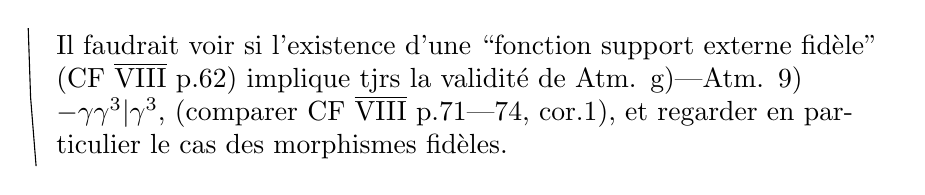
\begin{tikzpicture}
\node[anchor=north west,inner sep=0pt,text width=0.88\linewidth] (opening) at (0,0) {Il faudrait voir si l'existence d'une ``fonction support externe fidèle'' (CF \uline{$\overline{\mathrm{VIII}}$} p.62) implique tjrs la validité de \unsure{Atm. g)|Atm. 9)} $-\unsure{\gamma\gamma^3|\gamma^3}$, (comparer CF \uline{$\overline{\mathrm{VIII}}$} p.\unsure{71|74}, cor.1), et regarder en particulier le cas des \unsure{morphismes} fidèles.};
\draw ([xshift=-0.35cm,yshift=0.08cm]opening.north west) -- ([xshift=-0.32cm]opening.west);
\draw ([xshift=-0.32cm]opening.west) -- ([xshift=-0.25cm,yshift=-0.08cm]opening.south west);
\end{tikzpicture}}

Mais avant tout, il me faudrait aller de l'avant, pour me rendre compte exactement comment vont intervenir les axiomes des supports, et s'ils \deleted{sont}\inserted{s'avèrent} aussi cruciaux que je le pressens.

\figure{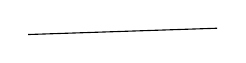
\begin{tikzpicture}\draw (0,0) -- (2.4,0.08);\end{tikzpicture}}

Critique philosophique de cette approche vers les supports, via les ``spatios'' ou ``\unsure{espacons|espaces}''. Dans la définition même des opérations essentielles $\unsure{\operatorname{co\!-\!sup}^{0}|\operatorname{co\!-\!sup}^{\circ}}$, $\unsure{\perp|\lrcorner}-\operatorname{sup}^{0}$, on est forcé de ``composer'' des strates qui ne sont pas néc. compatibles, ni même ``commensurables'' (\unsure{spectralement} disons, et encore moins combinatoirement). Or il semble \unsure{qu'on|qu'en}
